\documentclass{article}
\usepackage{graphicx} % Required for inserting images
\usepackage[%  
    colorlinks=true,
    pdfborder={0 0 0},
    linkcolor=red
]{hyperref}
\usepackage{geometry}
 \geometry{
 a4paper,
 total={173mm, 247mm},
 left=18mm,
 top=20mm,
 }

\title{Brew Bucks - diff22}
\author{Nimesh Garg, Peidong Liu, Lars Moan, Daniel Morgan, Manav Trivedi, Sai Karthikeya Vermulapalli}
\date{April 27, 2024}

\begin{document}

\maketitle
\pagebreak

\tableofcontents
\pagebreak

\section{Abstract}
Summarise the key points of your document.
\section{Changes}
Describe and justify any changes made to the project from what was outlined in the proposal.

\subsubsection*{1. Add Simplicity Quality Attribute}
There are items below that correspond to features under the functionality section in the original proposal. The items indicate why simplicity is relevant to the application.

\medskip \begin{minipage}{\dimexpr\textwidth-0.25cm}
1. Extensive Coffee Menu 
\begin{itemize}
    \item Desire for customers to explore a range of foods with ease
    \item A user-friendly interface for the menu is recognised
    \item Categorised browsing for 'easy' navigation through menu items
\end{itemize}

3. Easy Payments
\begin{itemize}
    \item Feature is regarded as something that is easy to perform or in other words, simple
\end{itemize}

5. Reward Points and Loyalty Program
\begin{itemize}
    \item Customers should view accumulated points with ease
    \item Raises the need to design navigation, UI and feature interaction to be simple
\end{itemize}
\end{minipage}

\bigskip \noindent The features above reflect the need for simplicity in the application. However, there currently isn't a quality attribute to bring this to the forefront of a developer's attention. Consequently, it is likely to be overlooked through the project's implementation. The team decided to approach this problem by establishing simplicity as a quality attribute. Ideally, this will encourage simple solutions to problems encountered when developing Brewbucks, just as the author implies. This goes for the architecture, features and UI. This feels justified given the proposal's author has emphasised the need for customers to engage with the platform with ease. Therefore, simplicity can be regarded as an obvious, yet neglected quality attribute. 



\section{Architecture Options}
What architectural design patterns were considered and their pros and cons.

\subsection{Event-Driven Architecture}
\subsubsection*{Pros for System Functionality}
\begin{itemize}
    \item Asynchronous communication can help with taking orders and processing payments concurrently
    \item Event handler cohesion principle can be used to scale for high load tasks, such as taking orders and processing payments
    \item Broker topology is suitable for sequential events, e.g., take coffee order, handle payment, make coffee, finish order
\end{itemize}
\subsubsection*{Cons for System Functionality}
\begin{itemize}
    \item Asynchronous communication and the inevitable communication failures add to architecture complexity
\end{itemize}

\subsubsection*{Pros for ASRs}
\begin{itemize}
    \item Broker topology is simple to implement and optimised for performance, responsiveness, scalability, extensibility, fault tolerance and low coupling
    \item Event handlers can be scaled to better manage their load through a load balancer and automated scaling mechanism
    \item Libraries and cloud-computing platforms make it easier to implement underlying functionality of event broker
    \item Have a channel implement a queue for scalability
\end{itemize}
\subsubsection*{Cons for ASRs}
\begin{itemize}
    \item It can be a challenge to implement event handlers so that they don't rely on event broker's deployment structure.
    \item Testing and debugging is hard with asynchronous communication
    \item When recoverability is compromised, implementing the broker topology is hard (bad for availability)
    \item Development team unfamiliar with supporting libraries and services
    \item Implementing event-driven architecture is complex
\end{itemize}

\subsection{Microservices Architecture}
\subsubsection*{Pros for System Functionality}
\begin{itemize}
    \item Application is suited to independently deployable, loosely coupled, components, e.g., a service for orders, payment, tracking, rewards
    \item Can distribute operations asynchronously using a message broker - helps with taking orders and processing payments concurrently
\end{itemize}   
\subsubsection*{Cons for System Functionality}
\begin{itemize}
    \item Operations may need to be implemented with complex, non-ACID transaction management (loose coupling requires services to have independent databases)
    \item Risk of tight design-time coupling between services, which means time consuming lockstep changes
    \item Design challenges with implementing distributed operations
\end{itemize}

\subsubsection*{Pros for ASRs}
\begin{itemize}
    \item Services can consist of a small number of subdomains - makes for greater simplicity, understanding and maintainability
    \item Different services can use different technology stacks and can be upgraded independently (extensibility)
    \item Subdomains can be split by concerns for separate services - supports scalability, availability, security etc
\end{itemize}
\subsubsection*{Cons for ASRs}
\begin{itemize}
    \item Maintainability affected by complex distributed operations, making troubleshooting trickier
    \item Availability affected by distributed operations with tight runtime coupling between services
    \item Implementing a microservices architecture is complex
\end{itemize}

\subsection{Brewbucks Architecture Justification}
\subsubsection*{Pros for System Functionality}
\begin{itemize}
    \item Shared database offers data integrity and consistency. It's needed for reliable order tracking, history and rewards
    \item Food Purchasing service can manage all database transactions for placing an order, e.g., when a food is no longer available, the service can rollback the transaction to guarantee data integrity (supports reliability)
\end{itemize}
\subsubsection*{Cons for System Functionality and ASRs}
\begin{itemize}
    \item Cons (and justification for these) are discussed in section 5 Trade-offs 
\end{itemize}

\subsubsection*{Pros for ASRs}
\begin{itemize}
    \item Simple, flexible, distributed architecture
    \item Domain partitioning offers high-level modularity 
    \item Domain distribution supports multiple instances of a service using a load balancer, enabling greater availability and some scalability 
    \item Service design locator pattern used to provide easier extensibility
    \item Stateless service pattern for multiple running instances of a service offers greater reliability
    \item All services can use the same façade design pattern for simplicity
    \item Support for the independent service principle makes for a simple, maintainable, deployable and modular design
\end{itemize}

\medskip \noindent \textbf{Simplicity QA}
\hfill \break Remember that simplicity is a newly introduced quality attribute. To achieve this, the principle of KISS was followed when developing Brewbucks. This idea applies especially when approaching the architecture for the project. To meet the desired quality attributes, a simple solution can be adopted with slight enhancements. As it stands, the event-driven and microservices architecture do not pursue a simple solution. A complex solution also becomes less feasible when the project's time constraints are considered. More to this, the development team felt that microservices would introduce complications associated with implementing distributed operations and tight design-time coupling between services. While event-driven would bring challenges in trying to successfully implement the event and worker queues.

\medskip \noindent \textbf{Well Satisfied QAs}
\hfill \break Service based architecture does well to meet several quality attributes. This includes: availability, reliability, extensibility, testability and deployability. Testability has been given higher priority for this project as evaluation is a key part of the delivery. Note that event-driven architecture falls short here as there are complications in testing and debugging asynchronous communication. Meanwhile, microservices introduces some complexity when trying to understand the call chain for any given request. Several microservices would not be easy to understand, hindering the application's maintainability and testing. Service-based architectures limits the number of network calls as it groups largers chunks of code together by domain (will boost performance) (Fletcher, 2016).

\medskip \noindent \textbf{Partially Satisfied QAs}
\hfill \break Conversely, there are quality attributes only partially met: interoperability, security and scalability. Scalability levels are considered sufficient for coffee orders. In a one hour period, it's expected that the app will receive 100 - 115 orders (Coffee School, 2022). See the testing evaluation for a summary of how the app performed under such conditions. Interoperability can be achieved with the API abstraction principle. Additional security support can be added by using an API layer to add security policies.

\hfill \break For these reasons, the team felt that the service-based architecture balances functionality, quality attributes and project constraints quite well.  

\section{Architecture}
Brewbucks software architecture description.

\begin{figure}
    \centering
    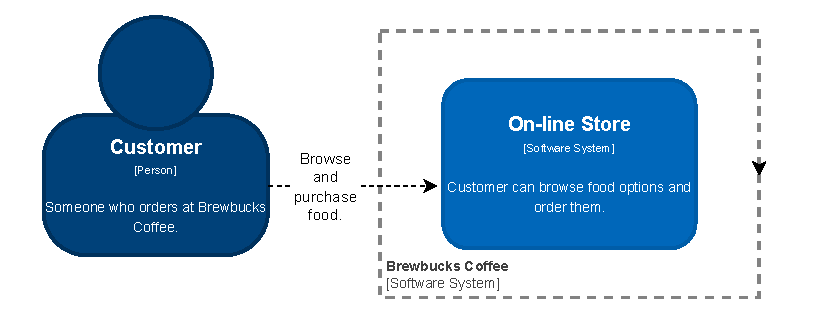
\includegraphics[width=0.5\linewidth]{model/c4/pdf/context_drawio.pdf}
    \caption{Context Diagram}
    \label{fig:context}
\end{figure}

\subsubsection*{General Overview of Architecture}
\medskip \noindent Application has a service-based architecture
\begin{itemize}
    \item Five distributable services based on app's core functionality (see figure \ref{fig:container})
    \begin{itemize}
     \item Supports features such as viewing menu items, payments, order history and status, reward point system
     \item Easily extensible for new features
     \item Domain partitioning offers high-level modularity and deployability
     \item Enables multiple instances of a service using a load balancer for greater availability and some scalability
   \end{itemize}
   \item Service APIs implemented for interoperability support
   \item Shared database for all containers 
    \begin{itemize}
     \item Supports reliability by ensuring data integrity and consistency
    \end{itemize}
   \item Services don't retain any state from previous calls - stateless service pattern
    \begin{itemize}
    \item Offers higher reliability, in terms of running multiple instances of a service
    \item  Request calls are designed so that information on whose details are asked for, are provided. Calls are /users/\{userid\}/orders/\{orderid\}/items as opposed to /items.
     \item Example? Food Purchasing service is responsible for finalising an order by accepting payment. Say there are 10 instances for Food Purchasing service, it doesn't matter which instance serves the request, customer always gets same data. Consequently, instances can scale up and down as needed.
     \item Handle traffic for Brewbucks application with load balancer
    \end{itemize}
    \item Check the status of instances with a healthcheck through AWS EC2 (maintainability and testing support)
    \item Service-based principles encourage a simple, maintainable, deployable and modular design
    \begin{itemize}
     \item Independent service principle is followed whereby none of the services depends on another
    \end{itemize}
\end{itemize}

\subsubsection*{Key Observations \ref{fig:container}} 
\begin{itemize}
    \item The single database server with logical partitioning of the data satisfies the system in terms of performance. Examples of partitioning include payments and reward-points table
    \item A separate user interface was implemented for employee accounts to change a customer's order status
    \item Domain services are not used by external systems, so a reverse proxy was not necessary. Payment service has a simple implementation as opposed to using an external payment provider 
\end{itemize}

\subsubsection*{Design Problem Consideration}
\bigskip \hfill \begin{minipage}{\dimexpr\textwidth-0.5cm}
\textbf{1. Shared database complications:} More services makes the database design more complicated. Performance bottlenecks may occur. 

\medskip \textbf{Solution?} User interface will not be complicated as there are only five services. Database design was relatively simple given this app can be treated as a small-sized system. It's expected that coffee orders are 100 - 115 in a 1 hour busy period. See 7 Evaluation for more.
\end{minipage}

\newgeometry{left=1.5cm,bottom=2.0cm,right=1.5cm,top=2.0cm}
\begin{figure}
    \centering
    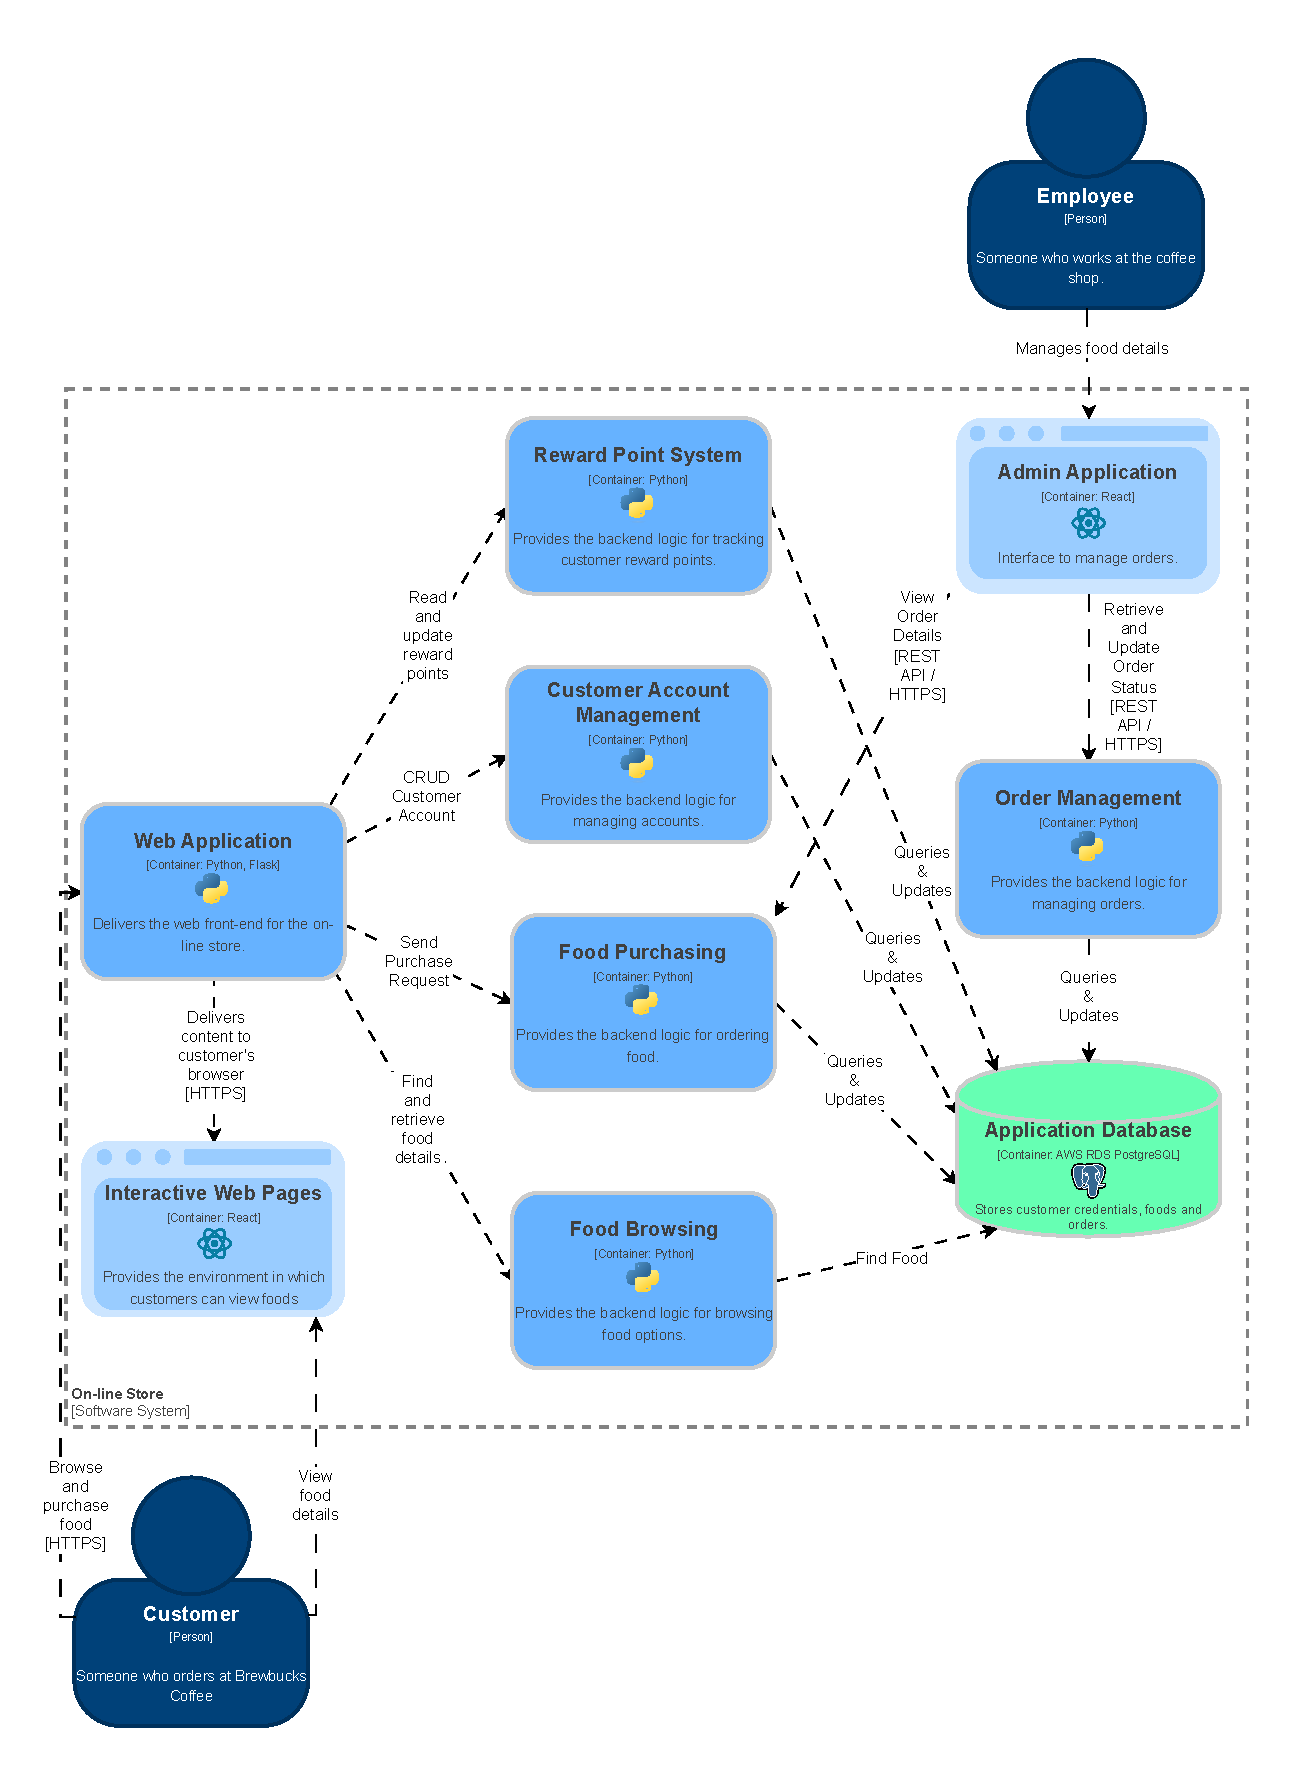
\includegraphics[width=0.80\linewidth]{model/c4/pdf/on-line-store-container-diagram_drawio.pdf}
    \caption{Container Diagram}
    \label{fig:container}
\end{figure}
\begin{figure}
    \centering
    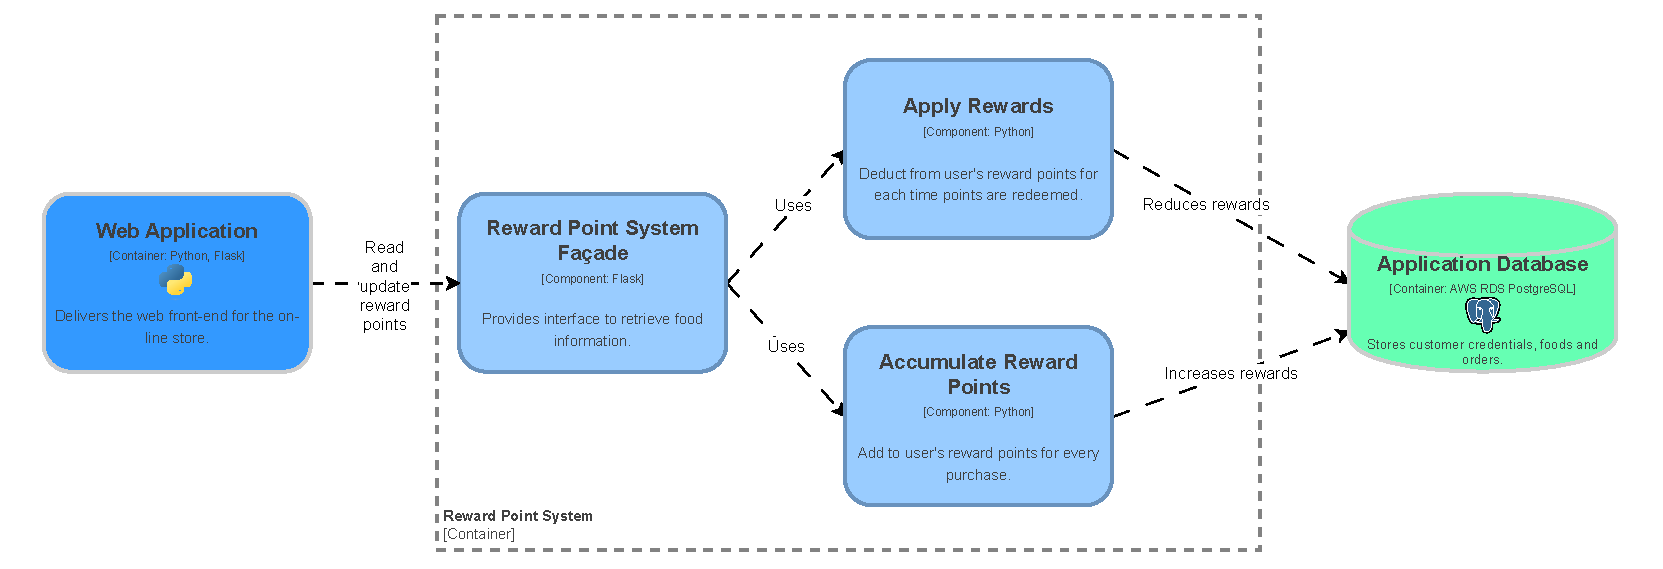
\includegraphics[width=1.0\linewidth]{model/c4/pdf/reward_point_system_drawio.pdf}
    \caption{Reward Point System Component Diagram}
    \label{fig:rewards}
\end{figure}
\begin{figure}
    \centering
    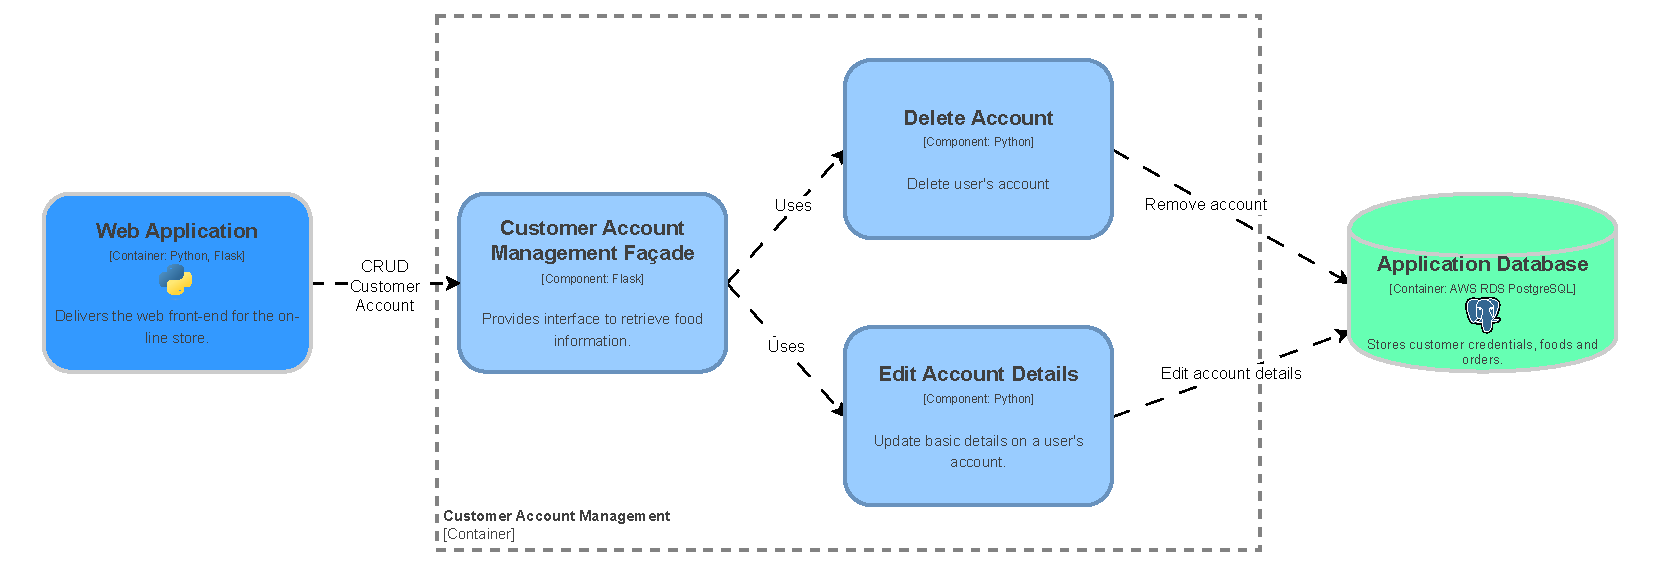
\includegraphics[width=1\linewidth]{model/c4/pdf/customer_account_management_drawio.pdf}
    \caption{Customer Account Management Component Diagram}
    \label{fig:customer}
\end{figure}
\begin{figure}
    \centering
    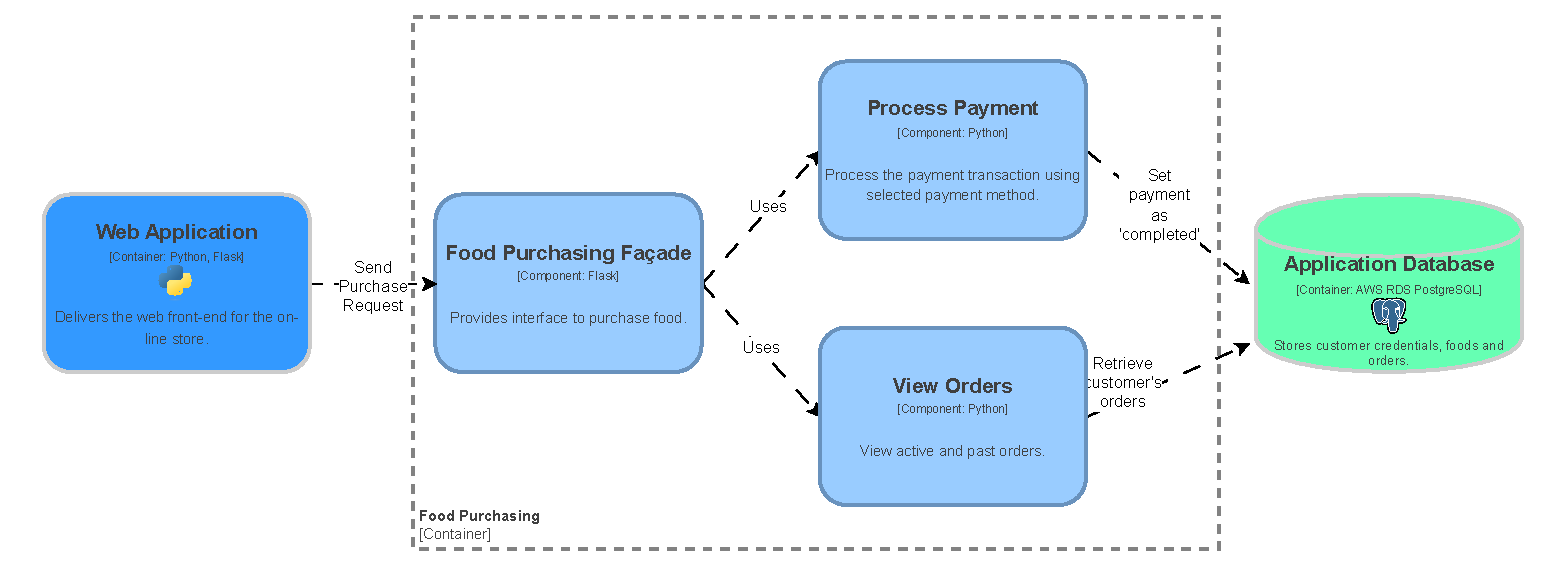
\includegraphics[width=1\linewidth]{model/c4/pdf/food_purchasing_drawio.pdf}
    \caption{Food Purchasing}
    \label{fig:purchase}
\end{figure}
\begin{figure}
    \centering
    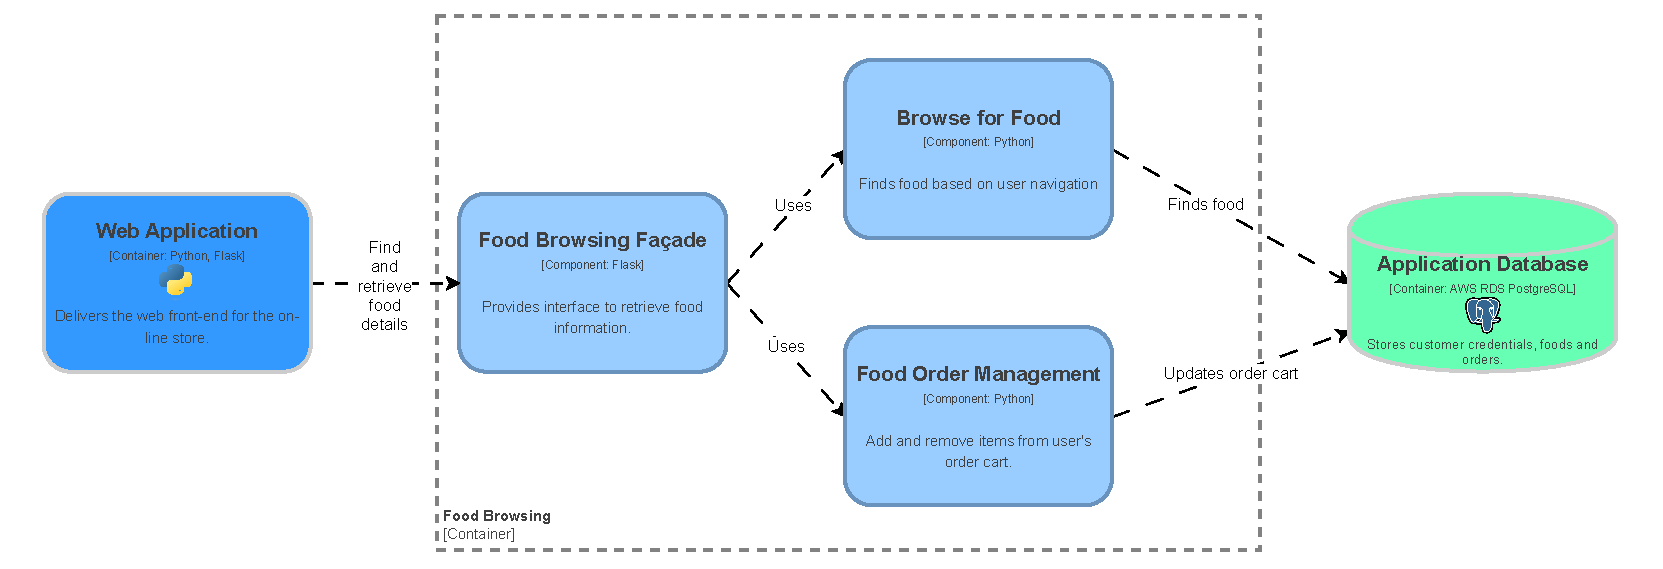
\includegraphics[width=1.0\linewidth]{model/c4/pdf/food_browsing_drawio.pdf}
    \caption{Food Browsing Component Diagram}
    \label{fig:browse}
\end{figure}

\begin{figure}
    \centering
    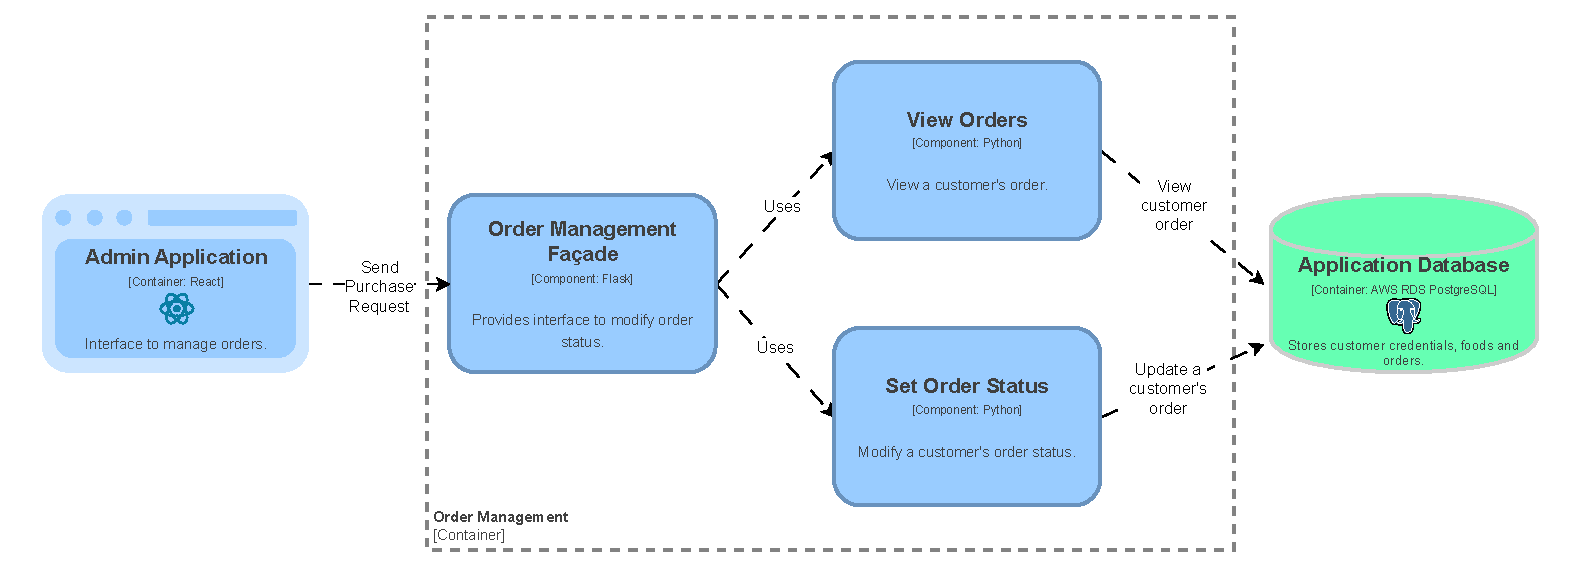
\includegraphics[width=1.0\linewidth]{model/c4/pdf/order_management_drawio.pdf}
    \caption{Order Management Component Diagram}
    \label{fig:orders}
\end{figure}
\restoregeometry






\section{Trade-Offs}
Describe and justify the trade-offs made in designing the architecture.
\section{Critique}
Describe how well the architecture supports delivering the complete system.
\section{Evaluation}
Summarise testing results and justify how well the software achieves its quality attributes.
\section{Reflection}
Lessons learnt and what you would do differently.

\section{References}
\par \sloppy Coffee School. (2022, July 6). How Many Coffees Can a Barista Make in an Hour? – Coffee School. https://www.coffeeschool.com.au/news/how-many-coffees-can-a-barista-make-in-an-hour
\par Fletcher, M. (2016, October 7). Service-Based Architecture as an Alternative to Microservice Architecture. InfoQ. https://www.infoq.com/news/2016/10/service-based-architecture/
\par Richardson, C. (2019). Microservices Pattern: Microservice Architecture pattern. Microservices.Io. Retrieved May 28, 2024, from http://microservices.io/patterns/microservices.html

\footnote{Footnote}




\end{document}
